\documentclass{../notes}

\title{决策理论 HW04}

\loadgeometry{word-narrow}

\begin{document}
    \maketitle

    \paragraph*{1}

    根据题意,设采购帆布鞋的数量为$x$,则采购冬靴的数量为$100-x$,已知采购帆布鞋的总回报为$32x$,对于冬靴,其销售收益存在不确定性,设3月前的销量占总销量的占比为随机变量$Y\in [0, 1]$,对应的回报为$(22 + 16y)(100 - x) = (2200 + 1600y) - (22x + 16xy)$。因此,总的回报为

    \begin{derive}[g(x, y)]
        &= 32x + (2200 + 1600y) - (22x + 16xy) \\
        &= (2200 + 1600y) + (10 - 16y)x
    \end{derive}

    由$x \geq 0, 100-x\geq 0$可知$x\in [0, 100]$。假设$Y$的分布函数为$\prob{y\leq Y} = F(y)$。

    \begin{subquestions}
        \item 当采用$\max_x\min_y$策略时,总回报为$g(x, 0) = 2200+10x$,$\arg\max _x g(x, 0) = 100$,因此$\max_x\min_y$策略为全部采购帆布鞋;
        \item 当采用$\max_x\max_y$策略时,总回报为$g(x, 1) = 3800-6x$,$\arg\max _x g(x, 1) = 0$,因此$\max_x\max_y$决策为采购冬靴。
        \item 当采用$\min_x\max\text{regret}_y$策略时,设后悔值定义为

        \begin{derive}[\rho(x, y)]
            &= \max_k g(k, y) - g(x, y) \\
            &= 3200 - (2200 + 1600y) + (10 - 16y)x \\
        \end{derive}

        因此$\min_x\max_y \rho(x, y) = \min_x (1000 + 10x)$,因此$\min_x\max\text{regret}_y$决策为采购冬靴。
    \end{subquestions}

    \paragraph*{2}

    \begin{subquestions}
        \item 决策树如图\ref{fig:dt-1}所示,下注Angel的期望收益为$0.7\times 1 + 0.3\times (-1) = 0.4$,下注Jack的期望收益为$0.1\times 10 + 0.9\times (-1) = 0.1$,因此最优决策为下注Angel,期望收益为$0.4$。

        \begin{figure}
            \centering
            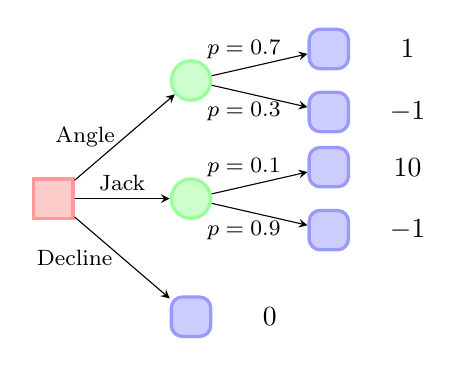
\begin{tikzpicture}
                [
                    DecisionNode/.style={rectangle, draw=red!40, fill=red!20, very thick, minimum size = 5mm},
                    ChanceNode/.style={circle, draw=green!40, fill=green!20, very thick, minimum size = 5mm},
                    ResultNode/.style={rectangle, rounded corners, draw=blue!40, fill=blue!20, very thick, minimum size = 5mm},
                    Connection/.style={-stealth},
                    Label/.style={font=\footnotesize}
                ]
                \node[DecisionNode](Root){};
                \node[ChanceNode, right of=Root, xshift=0.75cm, yshift=1.5cm](Angel){};
                \node[ChanceNode, right of=Root, xshift=0.75cm, yshift=0cm](Jack){};
                \node[ResultNode, right of=Root, xshift=0.75cm, yshift=-1.5cm](Decline){};
                \node[ResultNode, right of=Angel, xshift=0.75cm, yshift=0.4cm](Angel-Win){};
                \node[ResultNode, right of=Angel, xshift=0.75cm, yshift=-0.4cm](Angel-Lose){};
                \node[ResultNode, right of=Jack, xshift=0.75cm, yshift=0.4cm](Jack-Win){};
                \node[ResultNode, right of=Jack, xshift=0.75cm, yshift=-0.4cm](Jack-Lose){};

                \draw[Connection] (Root) -> node[left, Label] {Angle} (Angel);
                \draw[Connection] (Root) -> node[Label, yshift=0.2cm] {Jack} (Jack);
                \draw[Connection] (Root) -> node[left, Label] {Decline} (Decline);
                \draw[Connection] (Angel) -> node[Label, xshift=-0.2cm, yshift=0.2cm] {$p=0.7$} (Angel-Win);
                \draw[Connection] (Angel) -> node[Label, xshift=-0.2cm, yshift=-0.2cm] {$p=0.3$} (Angel-Lose);
                \draw[Connection] (Jack) -> node[Label, xshift=-0.2cm, yshift=0.2cm] {$p=0.1$} (Jack-Win);
                \draw[Connection] (Jack) -> node[Label, xshift=-0.2cm, yshift=-0.2cm] {$p=0.9$} (Jack-Lose);

                \node[right of=Decline]{$0$};
                \node[right of=Angel-Win]{$1$};
                \node[right of=Angel-Lose]{$-1$};
                \node[right of=Jack-Win]{$10$};
                \node[right of=Jack-Lose]{$-1$};
            \end{tikzpicture}
            \caption{决策树}
            \label{fig:dt-1}
        \end{figure}

        \item 决策树如图\ref{fig:dt-2}所示,下注Angel的期望收益为$0.7\times 2.5 + 0.3\times 2 = 2.35$,下注Jack的期望收益为$0.9\times 2 + 0.1\times 7 = 2.5$。当风险中性时,会选择下注Jack。

        \begin{figure}
            \centering
            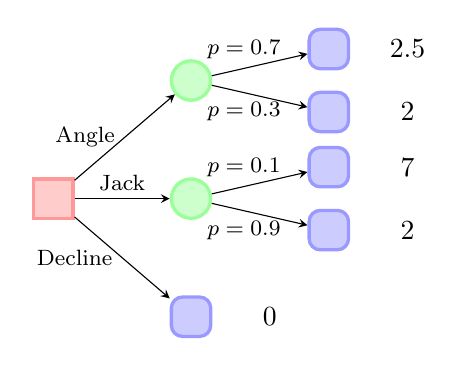
\begin{tikzpicture}
                [
                    DecisionNode/.style={rectangle, draw=red!40, fill=red!20, very thick, minimum size = 5mm},
                    ChanceNode/.style={circle, draw=green!40, fill=green!20, very thick, minimum size = 5mm},
                    ResultNode/.style={rectangle, rounded corners, draw=blue!40, fill=blue!20, very thick, minimum size = 5mm},
                    Connection/.style={-stealth},
                    Label/.style={font=\footnotesize}
                ]
                \node[DecisionNode](Root){};
                \node[ChanceNode, right of=Root, xshift=0.75cm, yshift=1.5cm](Angel){};
                \node[ChanceNode, right of=Root, xshift=0.75cm, yshift=0cm](Jack){};
                \node[ResultNode, right of=Root, xshift=0.75cm, yshift=-1.5cm](Decline){};
                \node[ResultNode, right of=Angel, xshift=0.75cm, yshift=0.4cm](Angel-Win){};
                \node[ResultNode, right of=Angel, xshift=0.75cm, yshift=-0.4cm](Angel-Lose){};
                \node[ResultNode, right of=Jack, xshift=0.75cm, yshift=0.4cm](Jack-Win){};
                \node[ResultNode, right of=Jack, xshift=0.75cm, yshift=-0.4cm](Jack-Lose){};

                \draw[Connection] (Root) -> node[left, Label] {Angle} (Angel);
                \draw[Connection] (Root) -> node[Label, yshift=0.2cm] {Jack} (Jack);
                \draw[Connection] (Root) -> node[left, Label] {Decline} (Decline);
                \draw[Connection] (Angel) -> node[Label, xshift=-0.2cm, yshift=0.2cm] {$p=0.7$} (Angel-Win);
                \draw[Connection] (Angel) -> node[Label, xshift=-0.2cm, yshift=-0.2cm] {$p=0.3$} (Angel-Lose);
                \draw[Connection] (Jack) -> node[Label, xshift=-0.2cm, yshift=0.2cm] {$p=0.1$} (Jack-Win);
                \draw[Connection] (Jack) -> node[Label, xshift=-0.2cm, yshift=-0.2cm] {$p=0.9$} (Jack-Lose);

                \node[right of=Decline]{$0$};
                \node[right of=Angel-Win]{$2.5$};
                \node[right of=Angel-Lose]{$2$};
                \node[right of=Jack-Win]{$7$};
                \node[right of=Jack-Lose]{$2$};
            \end{tikzpicture}
            \caption{决策树}
            \label{fig:dt-2}
        \end{figure}
    \end{subquestions}

    \paragraph*{3}

    影响图如图\ref{fig:dt-3}所示。

    \begin{figure}
        \centering
        \begin{tikzpicture}
            [
                DecisionNode/.style={rectangle, draw=red!40, fill=red!20, very thick, minimum size = 5mm},
                ChanceNode/.style={circle, draw=green!40, fill=green!20, very thick, minimum size = 5mm},
                ResultNode/.style={rectangle, rounded corners, draw=blue!40, fill=blue!20, very thick, minimum size = 5mm},
                Connection/.style={-stealth},
                Label/.style={font=\footnotesize}
            ]
            \node[DecisionNode, Label](Node1){Decision};
            \node[ResultNode, Label, right of=Node1, xshift=1cm](Node2){Outcome};
            \node[ResultNode, Label, right of=Node2, xshift=1cm](Node3){Payoff};

            \draw[Connection] (Node1) -> (Node2);
            \draw[Connection] (Node2) -> (Node3);

            \node[Label, below of=Node1]{选项:A、B};
            \node[Label, below of=Node2, yshift=-1cm]{
                \begin{tabular}{c}
                    概率 \\
                    $P(R=20|A) = 0.1$ \\
                    $P(R=10|A) = 0.2$ \\
                    $P(R=0|A) = 0.6$ \\
                    $P(R=-10|A) = 0.1$ \\
                    $P(R=5|B) = 0.7$ \\
                    $P(R=-1|B) = 0.3$ \\
                \end{tabular}
            };
        \end{tikzpicture}
        \caption{决策树}
        \label{fig:dt-3}
    \end{figure}

    \begin{enumerate}
        \item 选择A的期望回报为$0.1\times 20 + 0.2\times 10 + 0.1\times (-10) = 3$
        \item 选择B的期望回报为$0.7\times 5 + 0.3\times -1 = 3.2$
    \end{enumerate}

    由于选择B的期望回报高于选择A的期望回报,因此会选择B。
\end{document}